\laborator{Определение условий фазовых равновесий пар~-- жидкость}

\goal на основе экспериментальных данных по давлению насыщенных паров чистых компонентов определить условия фазовых равновесий пар~-- жидкость бинарной идеальной смеси при различных термодинамических условиях; результаты представить в виде диаграмм фазового равновесия ($у-х$; $Р-х, у$; $Т-х, у$).

\subsubsection{Теория}

В химической промышленности достаточно распространены процессы разделения газовых и жидких смесей, такие как ректификация, абсорбция, адсорбция и т.д. При проектировании процессов разделения данных систем необходимо иметь данные о равновесных свойствах рассматриваемых смесей. Условия фазового равновесия для наглядности удобно представлять в виде фазовой диаграммы, которая описывает влияние температуры, давления и состава на вид и число фаз, которые могут сосуществовать при данных условиях. Число фаз определяется согласно правилу фаз Гиббса. Вид фаз, которые могут сосуществовать в конкретных условиях, зависит от химической природы компонентов. Представление фазового равновесия более удобно в графическом виде, чем в табличном, так как позволяет охватить взаимные связи между переменными.

В соответствии с правилом фаз Гиббса для любой термодинамически равновесной системы число параметров состояния $С$ (степеней свободы), которые можно изменять, сохраняя число существующих фаз $Ф$ неизменным, определяется выражением
\begin{equation}
С=К-Ф+N,
\end{equation}
где $К$ – число компонентов системы, $N$ – число параметров состояния системы, имеющих одно и то же значение во всех фазах (обычно температура $Т$ и давление $p$, $N$ = 2). Величина $С$ определяет число параметров состояния, которые нужно задать для однозначного определения состояния системы.

Из правила фаз Гиббса следует, что в однокомпонентной системе ($К$ = 1) в однофазной области ($Ф$ = 1) состояние системы определяется двумя параметрами ($С$ = 2), например $Т$ и $p$.  Или другими словами, можно произвольно и одновременно изменять оба параметра до тех пор, пока система не окажется на одной из ограничивающих область линий фазового равновесия. На линиях фазового равновесия ($Ф$ = 2) состояние системы определяется одним параметром ($С$ = 1). Таким образом, произвольно можно менять только один из параметров, например $p$ или $Т$ (если изменяется $Т$, то $p$ будет изменяться в соответствии с ходом кривой, и наоборот). В трехфазной области ($Ф$ = 3) число степеней свободы равно нулю ($С$ = 0), что соответствует тройной точке, в которой ни один из параметров не может быть изменен, равновесное сосуществование трех фаз однокомпонентной системы возможно только при строго определенных значениях $Т$ и $p$, при изменении одного из состояний системы в тройной точке количество фаз уменьшится. Для любой системы число фаз максимально, когда $С$ = 0. При увеличении числа компонентов $К$ в системе растет число параметров состояния $С$, необходимых для однозначного определения состояния системы.

Для однокомпонентной системы в условиях равновесия двух фаз число степеней свободы число степеней свободы равно единице. Соответственно на двухкоординатной фазовой диаграмме условия фазового равновесия будут выглядеть в виде линии. В качестве примера на рисунке \ref{fig:phase-id.f1} представлена фазовая диаграмма и линии равновесия пар~-- жидкость, твердое~-- жидкость. Для двухкомпонентной системы при условиях фазового равновесия число степеней свободы равно двум. Представить условия фазового равновесия графически, с использованием двух координат, можно только зафиксировав одну из характеристик системы. 
\begin{figure}
	\begin{center}
		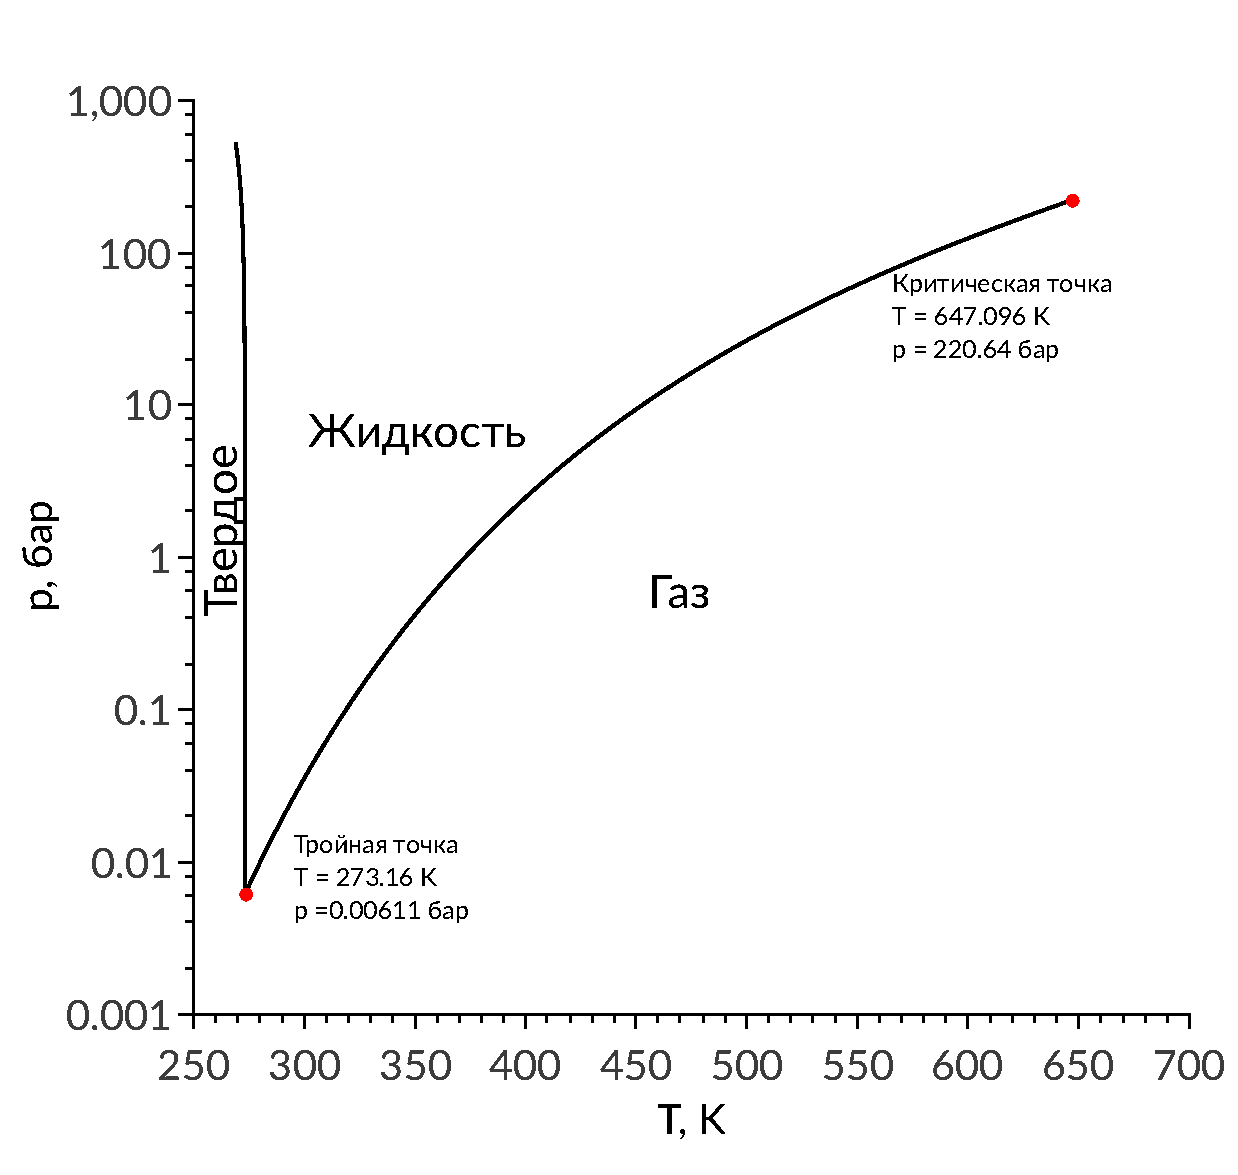
\includegraphics[width=0.6\textwidth]{phase-water.pdf}
	\end{center}
	\caption{Двухкоординатная фазовая диаграмма воды} \label{fig:phase-id.f1}
\end{figure}

Обычно используют следующие виды диаграмм, примеры приведены на рисунке \ref{fig:phase-id.f4}:
\begin{itemize}
	\item $p – x,y$ диаграмма строится при фиксированной температуре, и демонстрирует влияние давления и состава смеси на состояние фаз системы; 
	\item $T – x,y$ диаграмма строится при фиксированном давлении, и демонстрирует влияние температуры и состава смеси на состояние фаз системы;
	\item $x – y$ диаграмма демонстрирует зависимость между составами газовой и жидкой фаз.	
\end{itemize} 



\begin{figure}
	\begin{center}
		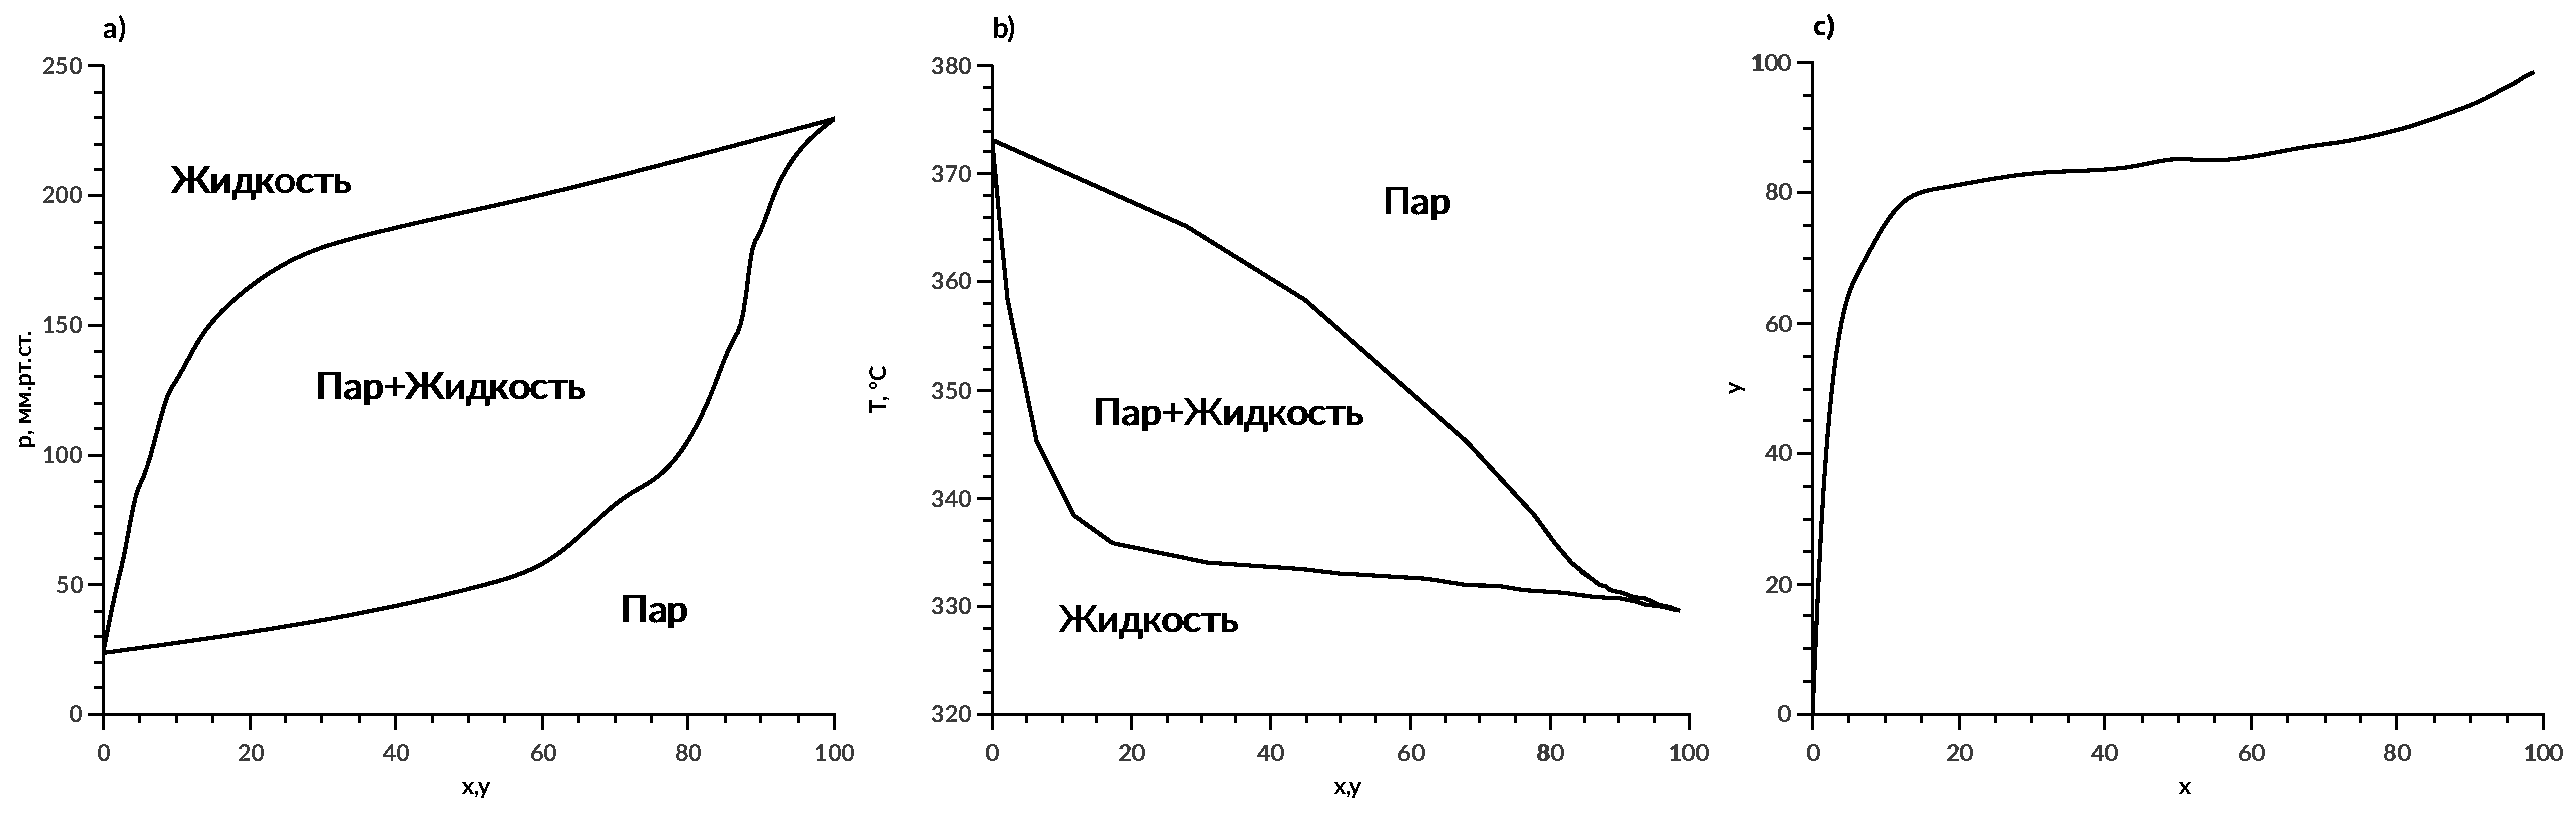
\includegraphics[width=1.0\textwidth]{phase-binary.pdf}
	\end{center}
	\caption{Фазовые диаграммы смеси ацетон"=вода a) $p - х, у$ при $T = 298 K$; b) $Т - х, у$ при $p = 760 мм.рт.ст.$; c) $y - x$ при $p = 760 мм.рт.ст.$} \label{fig:phase-id.f4}
\end{figure}

Для технических расчетов наиболее важной является диаграмма $Т – х, у$ --- зависимость температур кипения жидкости и конденсации паров от составов жидкой и паровой фаз, так как процессы перегонки в промышленных аппаратах протекают в изобарных условиях. 

Для проведения расчетов использование данных о фазовом равновесии в графическом виде не всегда удобно, особенно для многокомпонентных смесей. В этой связи условия фазовых равновесий удобно представлять в виде системы уравнений, решение которой позволит определить искомые параметры равновесия. 


\subsubsection{Определение условий фазового равновесия}
Условия равновесия двух фаз $n$--компонентной системы при заданной температуре $T$ определяются следующей системой уравнений:
\begin{equation}\label{eq:phas.equi}
\left\lbrace 
\begin{gathered} 
T^{I}=T^{II},\\
p^{I}(T,x_1,x_2,...,x_{n-1})=p^{II}(T,y_1,y_2,...,y_n-1),\\
\mu_i^{I}(T,x_1,x_2,...,x_{n-1})=\mu^{II}_i(T,y_1,y_2,...,y_n-1),
\end{gathered} 
\right.
\end{equation}
где $\mu^I_i$ --- химический потенциал (верхний индекс обозначает фазу, нижний --- компонент), $x$ --- мольная доля компонента в жидкой фазе, $y$ --- мольная доля компонента в газовой фазе. Чтобы определить условия фазового равновесия, необходимо решить систему уравнений \eqref{eq:phas.equi}. Численное решение данной системы можно получить, если выражения для химического потенциала и давления представлены в явном виде.
В однокомпонентном случае химический потенциал определяется следующим образом:
\begin{equation}
\int\limits_{\mu^0}^{\mu} d \mu=\dfrac{1}{N} \int\limits_{p^0}^{p} Vdp.
\end{equation}

Отсюда можно получить явный вид для химического потенциала, однако это возможно только если известно уравнение состояния. В случае использования уравнения состояния идеального газа $pV=NRT$ выражение будет иметь вид:
\begin{equation} \label{eq:phase.muid}
	\mu(T,p)=\mu^0(T)+RT \ln (p),
\end{equation}
где $\mu^0(T)$ --- химический потенциал идеального газа при единичном давлении. В случае смеси выражение \eqref{eq:phase.muid} будет иметь следующий вид:
\begin{equation} \label{eq:phase.muidi}
	\mu_i (T,p,x) = \mu_i^0(T) + RT \ln(p_i),
\end{equation}
где $p_i=p y_i$ --- парциальное давление компонента $i$ в газовой смеси.

Для систем, не подчиняющихся уравнению идеального газа вводится понятие летучести (фугитивности): $f_i=p_i \gamma_{f_i}$, где $\gamma_f$ --- коэффициент летучести (фугитивности), который зависит от $T$, $p$ и состава в случае смеси. Выражение для химического потенциала в этом случае запишется следующим образом:
\begin{equation} \label{eq:phase.mureal}
	\mu_i (T,p,x) = \mu_i^0(T) + RT \ln(f_i).
\end{equation}
В случае идеального газа $\gamma_f=1$.
Выражения \eqref{eq:phase.muid} -- \eqref{eq:phase.mureal}  записаны в случае, когда в качестве системы отсчета для химического потенциала выбрано состояние идеального газа $\mu^0(T)$, что не всегда удобно. Кроме того, коэффициент летучести (фугитивности) может быть определен, только если известно уравнение состояния реального вещества. 

В качестве системы отсчета для жидких смесей часто выбирают химический потенциал чистой жидкости  при тех же $p$ и $T$, что и смесь. В этом случае выражение химического потенциала для жидкой смеси запишется в виде:
\begin{equation}
	\mu_i(T,p,x)=\mu_i^0(T,p)+R T \ln (a_i),
\end{equation}
где $а_i$ --- активность, величина, учитывающая концентрационную зависимость химического потенциала компонентов реального раствора:
\begin{equation}
	a_i=\gamma_i x_i,
\end{equation}
где $\gamma_i$ --- коэффициент активности компонента $i$, в случае идеального раствора $\gamma_i =1 $.

Необходимо отметить, что стандартная часть химического потенциала (первое слагаемое) не зависит от концентрации (см. уравнения \eqref{eq:phase.muid} -- \eqref{eq:phase.mureal} ), концентрационная зависимость учитывается вторым слагаемым.

Теперь первое уравнение условий фазового равновесия пар~-- жидкость \eqref{eq:phas.equi} можно записать в виде:
\begin{equation}
	\mu_i^0(T)+RT \ln (f_i)=\mu_i^0(T,p)+ R T \ln (a_i),
\end{equation}
откуда после преобразований можно получить следующее выражение, связывающее концентрации компонента в фазах:
\begin{equation} \label{eq:phase.yreal}
	y_i=\dfrac{f_i^0 \gamma_i x_i}{\gamma_{f_i} p},
\end{equation}
где $f_i^0$ --- летучесть (фугитивность) чистого компонента $i$ при заданных $Т$ и $p$. 
По правилу фаз Гиббса n-компонентная двухфазная система имеет $n$ степеней свободы:
\begin{equation*}
	С=К-Ф+2=n-2+2=n.
\end{equation*}

Для $n$ независимых параметров, полностью определяющих состояние системы, обычно выбирают $n-1$ концентраций в жидкой фазе и $p$ или $Т$.

Следовательно, для определения состава паровой	 фазы и $p$ достаточно системы, состоящей из $n$ уравнений вида \eqref{eq:phase.yreal}, определяющих концентрации в паровой фазе, дополненной выражением:
\begin{equation}
	\sum\limits_{i=1}^{n} y_i =1.
\end{equation}

Данная система уравнений может быть упрощена, если принять, что:
\begin{itemize}
	\item паровая фаза подчиняется  уравнению состояния идеального газа, т.е. ${\gamma_f}_i =1$;
	\item при небольших давлениях значение летучести близко к давлению насыщенных паров чистого компонента $f_i^0 \approx p^0_i (T)$.
\end{itemize}
В итоге получим:
\begin{equation} \label{eq:phase.yapp}
y_i=\dfrac{p_i^0(T) \gamma_i x_i}{ p}.
\end{equation}
Систему уравнений \eqref{eq:phase.yapp} необходимо дополнить зависимостью коэффициента активности $\gamma_i$ от $T$, $p$ и состава, а также зависимостью давления насыщенных паров чистых компонентов от температуры $p^0_i(T)$. 

Для случая идеальной смеси ($\gamma_i=1$), находящейся в равновесии с идеальным паром, система \eqref{eq:phase.yapp} сводится к известному закону Рауля:
\begin{equation} \label{eq.phase.raoul}
	p_i=p_i^0(T) x_i.
\end{equation}

Общее давление для идеальной смеси в этом случае запишется в виде:
\begin{equation}\label{eq.phase.sump}
	p=\sum\limits_{i=1}^{n} p_i=  \sum\limits_{i=1}^{n} p_i^0 (T) x_i.
\end{equation}

\subsubsection{Модели для определения давления насыщенных паров чистых компонентов}


Для определения давления насыщенных паров чистых жидкостей используют различные корреляции \cite{yelles1989,rid1982}:
\begin{equation} \label{eq.phase.ant}
\left.
\begin{aligned} 
\text{Клапейрона} &\quad \ln(p_i^0(T))=A-\frac{B}{T};\\ 
Антуана &\quad \ln(p_i^0(T))=A-\frac{B}{T+C};\\ 
Риделя &\quad \ln(p_i^0(T))=A-\frac{B}{T}+C \ln(T)+D T^2;\\ 
Миллера &\quad \ln(p_i^0(T))=A-\frac{B}{T}+C T+D T^3;\\ 
Ренкина &\quad \ln(p_i^0(T))=A-\frac{B}{T}+С T^2;\\ 
Кеэгоу &\quad \ln(p_i^0(T))=A+\frac{B}{T}+С T+BT^2;\\ 
Реде &\quad \ln(p_i^0(T))=\frac{AT}{T+B}.
\end{aligned} 
\right\rbrace
\end{equation}
где $A$,$B$,$C$,$D$ --- параметры.

Решая систему уравнений \eqref{eq:phase.yapp} совместно с выражением для давления насыщенных паров \eqref{eq.phase.ant}, можно определить условия фазового равновесия системы жидкость ~-- пар для идеальной смеси, на основе которых можно построить соответствующие фазовые диаграммы. 
Алгоритм определения условий фазовых равновесий системы пар ~-- жидкость для идеальной смеси будет выглядеть следующим образом:
\begin{itemize}
	\item при $T = const$: определяют давления насыщенных паров чистых компонентов по одному из представленных выше уравнений \eqref{eq.phase.ant}, через которые, по выражению \eqref{eq.phase.sump} при известных концентрациях в жидкой фазе рассчитывают  $p$ в системе, а далее по выражению  \eqref{eq:phase.yapp} --- концентрации компонентов в паровой фазе;
	\item при $p = const$: необходимо определить температуру системы $Т$ при фиксированной концентрации компонентов в жидкой фазе путем решения нелинейного уравнения для общего давления в системе \eqref{eq.phase.sump} с учетом выражения для давления насыщенных паров \eqref{eq.phase.ant}. Далее по выражению \eqref{eq:phase.yapp} определяют концентрации компонентов в паровой фазе.
\end{itemize}

\subsubsection*{Модели для определения коэффициента активности}
Закон Рауля достаточно хорошо описывает свойства лишь небольшого количества смесей, например смеси легких углеводородов. В действительности же для реальных систем парциальное давление будет отличаться от давления, определенного по закону Рауля \eqref{eq.phase.raoul} и определяться выражением:
\begin{equation}
p_i=\gamma_i p_i^0(T) x_i,
\end{equation}
где  $\gamma_i$ --- коэффициент активности компонента i. Соответственно общее давление системы запишется в следующем виде:
\begin{equation} \label{eq.phase.pressgam}
p=\sum\limits_{i=1}^{n} p_i=\sum\limits_{i=1}^{n} \gamma_i p_i^0(T) x_i
\end{equation}

В этом случае для расчета условий фазового равновесия, кроме давления насыщенных паров чистого компонента при заданной температуре ($p_i^0(T)$), необходимо определить коэффициенты активности $\gamma_i$ в зависимости от температуры, давления и состава.
Коэффициенты активности определяют по данным экспериментальных измерений фазового равновесия ($p$, $T$, $х$, $у$) \cite{kogan1,kogan2} . При отсутствии этих экспериментальных данных коэффициенты активности также можно рассчитать, используя универсальные уравнения состояния, применимые как для жидкой, так и для паровой фазы. Однако в настоящее время подобные уравнения состояния охватывают лишь немногие группы веществ. Так, уравнения Соава и уравнения, аналогичные уравнению Бенедикта"=Уэбба"=Рубина, разработаны лишь для класса легких углеводородов и нескольких других газов \cite{rid1982}. Поэтому для определения коэффициентов активности широко используют различные модели.

Для корреляции коэффициентов активности с составом смеси, давлением и температурой предложено много уравнений \cite{rid1982,yelles1989}. Некоторые из них имеют более или менее разработанное теоретическое обоснование, другие являются чисто эмпирическими. В настоящее время наиболее известны пять основных видов корреляций коэффициентов активности (Маргулеса, Ван Лаара, Вильсона, NRTL, UNIQUAC). Поскольку преимущества какого"=либо одного метода не всегда явно выражены, на практике следует исходить из имеющегося опыта и аналогий. Также следует учитывать, что модели Маргулеса и Ван Лаара не подходят для описания многокомпонентных смесей.

Ниже для различных моделей приведены выражения избыточной энергии Гиббса и коэффициентов активности для двухкомпонентных смесей.
\begin{itemize}
	\item Модель Маргулеса.
	
	Выражение избыточной энергии Гиббса для двухкомпонентной смеси:
	\begin{equation}\label{eq.phase.gemarg}
	\frac{G^{ex}}{RT}=x_1 x_2 (A_{21} x_1+ A_{12} x_2),
	\end{equation}
	где $A_{12}$ и $A_{21}$ --- параметры модели.
	
	Выражения для коэффициентов активности:
	\begin{equation} \label{eq.phase.ga1marg}
	\ln(\gamma_1)=(A_{12}+2(A_{21}-A_{12})x_1)x_2^2,
	\end{equation}
	\begin{equation} \label{eq.phase.ga2marg}
	\ln(\gamma_2)=(A_{21}+2(A_{12}-A_{21})x_2)x_1^2.
	\end{equation}
	
	\item Модель ван Лаара.
	
	Выражение избыточной энергии Гиббса для двухкомпонентных смесей:
	\begin{equation}\label{eq.phase.gewlar}
	\frac{G^{ex}}{RT}=\dfrac{1}{\dfrac{1}{A_{12} x_1}+ \dfrac{1}{A_{21}x_2}},
	\end{equation}
	где $A_{12}$ и $A_{21}$ --- параметры модели.
	\begin{equation}
	\ln(\gamma_1)=A_{12}\left( \dfrac{A_{21}x_2}{A_{12}x_1 + A_{21} x_2}\right)^2,
	\end{equation}
	\begin{equation}
	\ln(\gamma_2)=A_{21}\left( \dfrac{A_{12}x_1}{A_{12}x_1 + A_{21} x_2}\right)^2.
	\end{equation}
	
	\item Модель Вильсона
	
	Выражение избыточной энергии Гиббса для двухкомпонентных смесей:
	\begin{equation}\label{eq.phase.wilson}
	\frac{G^{ex}}{RT}=-x_1 \ln(x_1+\Lambda_{12} x_2)-x_2 \ln(\Lambda_{21} x_1 +x_2)
	\end{equation}
	где $\Lambda_{12}=\frac{V_2^L}{V_1^L}\exp\left(-\frac{\lambda_{12}-\lambda_{11}}{RT} \right)$ и $\Lambda_{21}=\frac{V_1^L}{V_2^L}\exp\left(-\frac{\lambda_{21}-\lambda_{22}}{RT}\right)$,  $V_i^L$ --- молярный объем чистого компонента $i$, $\lambda_{ij}$ --- параметр, характеризующий силу взаимодействия компонентов $i$ и $j$ ($\lambda_{ij}=\lambda_{ji}$). 	В данной лабораторной работе можно использовать в качестве параметров $\Lambda_{12}$ и $\Lambda_{21}$, и в данном случае коэффициент активности будет зависеть только от состава жидкой фазы:
	
	\begin{equation}
	\ln(\gamma_1)=-\ln(x_1 + \Lambda_{12} x_2) + x_2 \left( \dfrac{\Lambda_{12}}{x_1 + \Lambda_{12} x_2 } - \dfrac{\Lambda_{21}}{\Lambda_{21} x_1+x_2} \right),
	\end{equation}
	\begin{equation}
	\ln(\gamma_2)=-\ln(x_2 + \Lambda_{21} x_1) + x_1 \left( \dfrac{\Lambda_{12}}{x_1 + \Lambda_{12} x_2 } - \dfrac{\Lambda_{21}}{\Lambda_{21} x_1+x_2} \right).
	\end{equation} 
	
	\item Модель NRTL (Non-Random Two-Liquid)
	
	Выражение избыточной энергии Гиббса для двухкомпонентных смесей:
	\begin{equation}\label{eq.phase.nrtl}
	\dfrac{G^{ex}}{RT}=x_1 x_2 \left( \dfrac{\tau_{21}G_{21}}{x_1 + G_{21} x_2} + \dfrac{\tau_{12} G_{12}}{G_{12} x_1 +x_2} \right),
	\end{equation}
	где $G_{12}=\exp(-\alpha_{12} \tau_{12})$,  $G_{21}=\exp(-\alpha_{21} \tau_{21})$, $\tau_{12}=\dfrac{g_{12}-g_{22}}{RT}$, $\tau_{21}=\dfrac{g_{21}-g_{11}}{RT}$, $g_{ij}$ --- параметр взаимодействия между компонентами i и j ($g_{ij}=g_{ji}$), $\alpha_{ij}$ --- параметр непроизвольности ($\alpha_{ij}=\alpha_{ji}$)
	В данной работе в качестве параметров модели можно использовать $\tau_{12}$,$\tau_{21}$, $\alpha_{12}$, в данном случае коэффициент активности будет зависеть только от состава жидкой фазы:
	\begin{equation}
	\ln(\gamma_1)=x^2_2 \left( \tau_{21} \left(\dfrac{G_{21}}{x_1+x_2 G_{21}}\right)^2 + \dfrac{\tau_{12} G_{12}}{(x_2+x_1 G_{12})^2} \right),
	\end{equation}
	\begin{equation}
	\ln(\gamma_2)=x^2_1 \left( \tau_{12} \left(\dfrac{G_{12}}{x_2+x_1 G_{12}}\right)^2 + \dfrac{\tau_{21} G_{21}}{(x_1+x_2 G_{21})^2} \right).
	\end{equation} 
\end{itemize}

Рассмотрим методику определения параметров бинарного взаимодействия в изотермическом случае. В качестве исходной информации выступают экспериментальные данные о фазовом равновесии пар – жидкость $(х, у, p, Т)$. Процедура определения параметров включает следующие этапы:
\begin{enumerate}
	\item При заданной температуре находят давления насыщенных паров чистых жидкостей $p_i^0(T)$, используя уравнения Менделеева~-Клайперона, Антуана, Риделя или др \eqref{eq.phase.ant}.
	\item Для всех имеющихся экспериментальных данных рассчитывают коэффициенты активности по выражениям:
	\begin{equation}
		\gamma_1=\dfrac{y_1 p}{x_1 p_1^0(T)},
	\end{equation}
	\begin{equation}
		\gamma_2=\dfrac{y_2 p}{x_2 p_2^0(T)}.
	\end{equation}
	\item По полученным значениям коэффициентов активности рассчитывают избыточную мольную энергию Гиббса $G^E$:
	\begin{equation}\label{eq.phase.expge}
		\dfrac{G^E}{RT}=x_1 \ln(\gamma_1)+x_2 \ln(\gamma_2).
	\end{equation}
	\item Используя  выражения для избыточной мольной энергии Гиббса (выражения \eqref{eq.phase.gemarg} \eqref{eq.phase.gewlar} \eqref{eq.phase.wilson} \eqref{eq.phase.nrtl} ) подбирают такие параметры моделей, чтобы минимизировать расхождение между значениями, рассчитанными по данным выражениям и экспериментальными данными \eqref{eq.phase.expge}.
\end{enumerate}

Для оценки точности полученных результатов обычно строят две диаграммы: $y – x$ и $p – x, у$ при некоторой постоянной температуре $Т$. Процедура построения включает следующие этапы на примере модели Маргулеса:
\begin{enumerate}
\item Используя уравнения \eqref{eq.phase.ga1marg} \eqref{eq.phase.ga2marg}, находят коэффициенты активности.
\item Для каждого выбранного значения $х$ находят соответствующее значение $p$ и $y$, используя выражения \eqref{eq.phase.pressgam} и \eqref{eq:phase.yapp}.
\item На основе полученных данных строят графические зависимости.
\end{enumerate}

\subsubsection*{Вопросы для самоконтроля:}
\begin{enumerate}
	\item Как формулируются условия фазового равновесия многокомпонентных многофазных систем?
	\item Как определяется число независимых параметров, полностью определяющих состояние системы?
	\item Какие существуют типы диаграмм фазового равновесия?
	\item Методы расчета фазовых равновесий при различных термодинамических условиях ($p-x,y$,  $T-x,y$).
	\item В каких случаях применим закон Рауля?
	\item Способы определения коэффициентов активности?
	\item Какие данные необходимы при определении параметров модели для описания коэффициентов активности?
\end{enumerate}

\subsubsection*{Пример задания}
\begin{enumerate}
	\item По экспериментальным данным (из справочника теплофизических свойств чистых веществ) получить описание зависимости давления паров чистого компонента от температуры. Для бензола использовать уравнение Антуана $ln(p_i^0(T))=A-\frac{B}{T+C}$         , для н-бутанола использовать уравнение Миллера $ln(p_i^0(T))=A-\frac{B}{T}+C T+DT^3$  . На основе полученных уравнений и закона Рауля, для смеси бензол--н-бутанол построить $p-x,y$ и $y-x$ диаграммы равновесия пар-жидкость при температуре   45.0 $^\circ$C . Сравнить результаты полученные по модели с экспериментальными данными и сделать вывод о применимости модели.
	
	\item Используя данные из предыдущего задания построить $T-x,y$ и $y-x$ диаграммы при давлении  760.0 мм.рт.ст. Сравнить результаты полученные по модели с экспериментальными данными \cite{kogan1,kogan2} и сделать вывод о применимости модели. 
	
	\item Используя данные из предыдущих заданий определить параметры уравнения Вильсона для описания коэффициента активности. Используя найденные значения параметров построить $T-x,y$ и $p-x,y$ диаграммы. Сравнить с результатом, полученным по уравнению Рауля.\end{enumerate}
